\chapter{The Limits of Depth Perception when Using Volumetric Illustrative Rendering Techniques} \label{chap:DepthPerception}
% What is this chapter looking into?
It has been shown that X-ray visualizations have improved the perceived depth mismatch caused by a visual misalignment when a virtual object is rendered behind a real object~\cite{Bajura1992, Avery2008, Sandor2010, Kalkofen2009}. 
\autoref{Chap:X-ray Implemntion} shows that \glspl{X-ray Visualization} techniques can impact depth perception, which is important to understand before they are proposed for activities that require precise hand-eye coordination tasks, especially activities like surgery. 
Occlusion is a powerful depth cue that uses virtual graphics to block physical world objects to influence the perceived depth. 
However, it can also obscure key information in some scenarios.
%Occlusion is a powerful depth cue but can obscure key details. 
The study presented in this chapter advances the current research knowledge by exploring the impact of \glspl{virt} on a user's depth perception when paired with \gls{dvr}.
%This study examines the impact of \glspl{virt} on a user's depth perception when paired with \gls{dvr}.

\begin{figure}[tb]
    \centering
    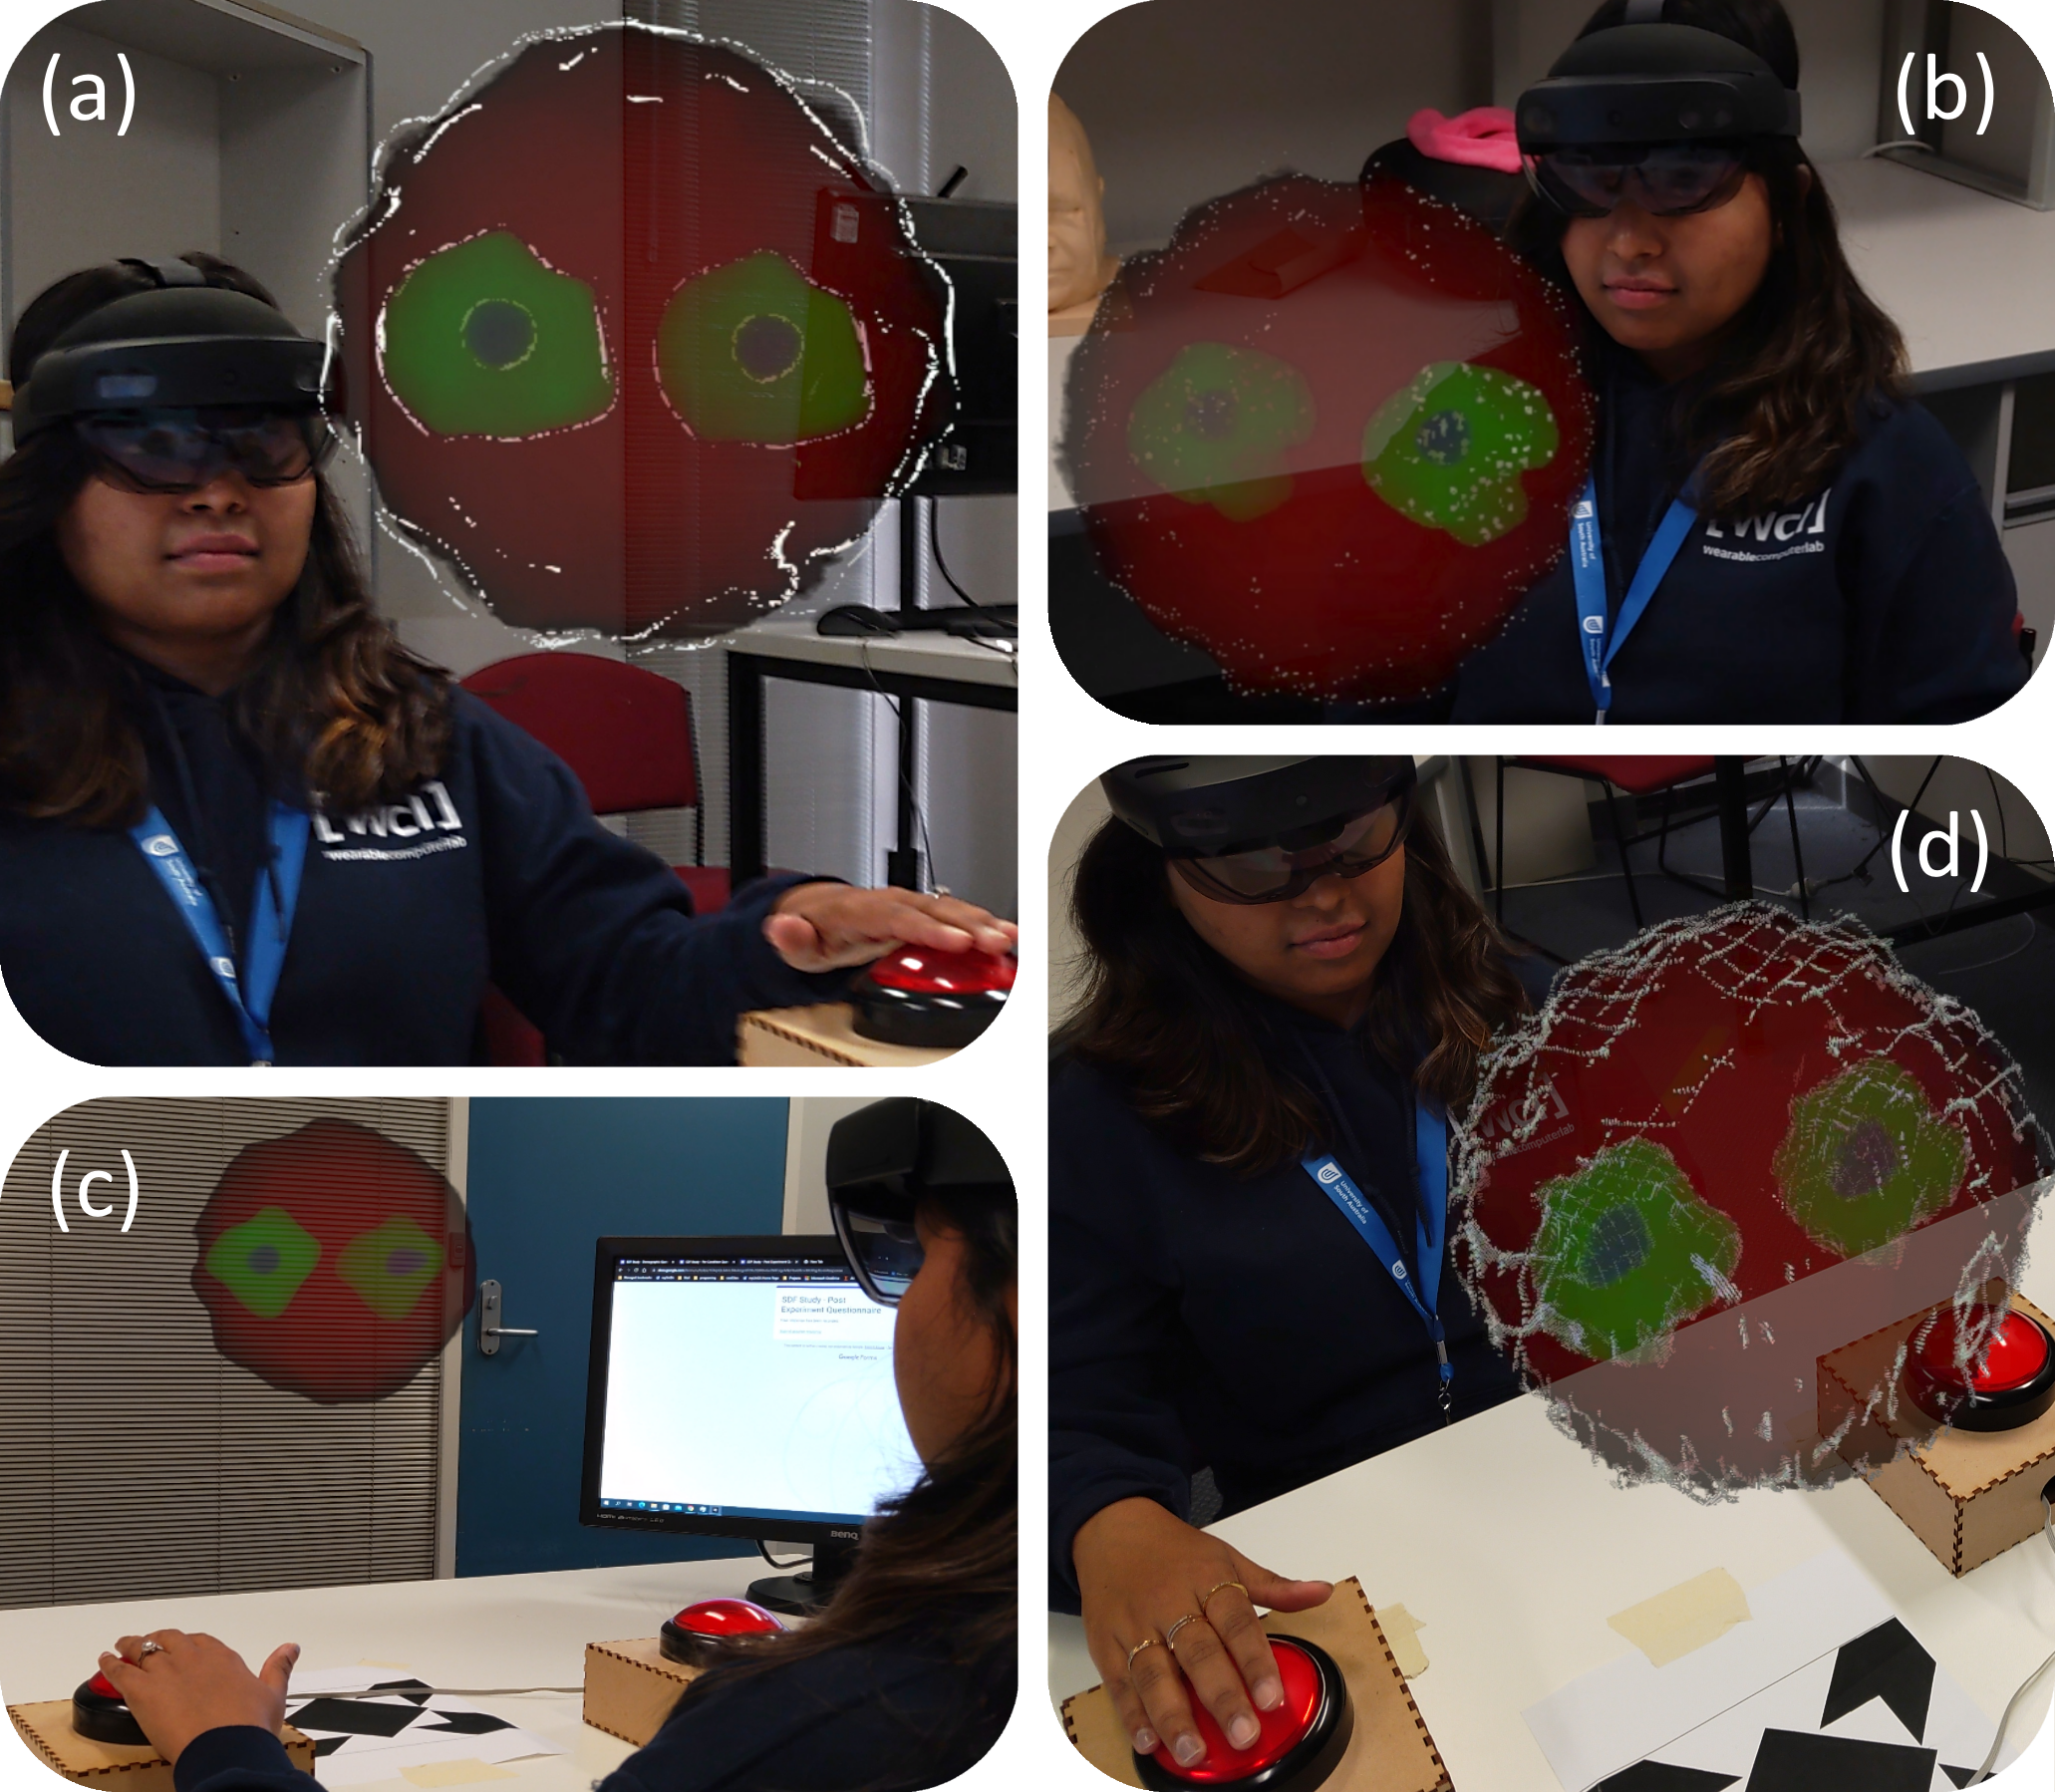
\includegraphics[width = \columnwidth]{Chapter6/Images/DepthPerceptionStudyPhotos.png}
    \caption[This figure shows the environment in which this study took place and presents each of the \gls{virt} conditions utalized in this study.]{This figure shows the environment in which this study took place and presents each of the \gls{virt} conditions utalized in this study. 
    All these images were taken using a HoloLens2 camera, viewing a user engaging with the study. 
    (a) Illustrates the \textit{Halo} \gls{virt} and shows a participant pressing one of the task buttons present in the study. 
    (b) Shows the \textit{Stippling} \gls{virt} being observed by the participant. 
    (c) Displays the \textit{No \gls{virt}} condition from the participant's perspective. 
    (d) Is an image of the \textit{Hatching} \gls{virt}.}
    \label{fig:DepthPerceptionPhotos}
\end{figure}

\gls{dvr} on desktop displays provides a good sense of depth when looking through an object. Our understanding of how it is affected when using a \gls{ar} \gls{hmd} is relatively unknown past the understanding that the previous devices struggled to run the visualizations efficiently enough~\cite{Sielhorst2006}.
Prior literature that focused on how humans understood how \glspl{virt} affects depth perception tends to include the following:
\begin{itemize}
    \item Spatial awareness is improved in VR when removing distracting details from the physical environment~\cite{Wijayanto2023};
    \item Illustrative geometric effects like those found in \gls{X-ray Vision} can better join the virtual world and the virtual world together by providing a clear reference where both of the relationship between them~\cite{Martin-Gomez2019};
    \item Illustrative effects are utilized in medical \gls{ar} as they are more tested at dealing with the depth mismatch when displaying structures that are located within each other since they can illustrate depth perception in ways that are not possible with transparency alone~\cite{Hansen2010, Lawonn2013};
    \item \autoref{fig:DepthPerceptionPhotos} Shows illustrative effects are also pleasing to see rendered inside of other objects as they are better designed to showcase ~\cite{Lawonn2017};
    \item Illustrative effects can convey curvature clearer than shaded meshes~\cite{Lowonn2013};
\end{itemize}
However, the literature has not discussed the impact of illustrative effects in tandem with \gls{dvr} regarding depth perception.
If \glspl{virt} are to be found useful for high-precision tasks, their accuracy with depth perception should not decrease depth perception and ideally improve or remove any mismatch.
\autoref{Chap:X-ray Implemntion}, demonstrated that having any \gls{X-ray Vision} effect impaired depth perception.
\autoref{Chap:VolumetricX-rayVision}, it was shown that both \textit{Stippling} and \textit{Hatching} may be detrimental to understanding the layout of a given volume.

This chapter's investigation required suitable methodologies to measure the impact of VIRTs, with the expectation that they would be used in a precise and stressful situation.
Similar to the study design used by Nagata~\cite{Nagata1983} and Chen et al.~\cite{Chen2018}, a \gls{twofc} psycho-physical experiment was conducted.
Nagata~\cite{Nagata1983} showed the participants an image or video displayed, either on an image, television, or stereoscopic display between two separate experiments to determine the impact of motion and stereopsis on depth perception.
The results from Nagata~\cite{Nagata1983} formed the foundations upon which a lot of depth perception research is based today, detailing the maximum thresholds of motion, binocular parallax, accommodation, and convergence while also stating some of the conditions that affect these factors.
Chen et al.~\cite{Chen2018} conducted a depth perception experiment examining the impact of binocular distortion using motion and focusing on creating depth cues that conflicted with each other by presenting slightly different phenomena in each eye showing that a more occlusive element would normally appear closer to the viewer if only shown in one eye.

% based on psycho-physical experimenting principles conducted, searching for the \gls{jnd} and \gls{pse} of the default volume rendering and all the \glspl{virt}.
% Due to the lack of similar literature in this area, it is first important for us to determine the thresholds where \gls{dvr} is able to provide.


% This chapter aims to determine the impact of using \glspl{virt} as an \gls{X-ray Visualization} to depth perception when compared to just using plan \gls{dvr} within a near field.
% The participant comments from \autoref{Chap:X-ray Implemntion} explained that participants struggled to notice if the \gls{X-ray Vision} effect was working or not due to their limited focus on the \gls{ost} \gls{ar} \gls{hmd}'s screen.
% So, this visualization was tested without \gls{X-ray Vision} as it would only distract the user from the algorithm they were performing. 

% %This chapter aims to Investigate the accuracy of depth perception that \glspl{virt} can achieve.
% %To ensure this is handled in the best possible way, we have designed this study to purely analyze the \gls{dvr} algorithm to accommodate a method of 
% By utilizing a study has been designed to evaluate how well \gls{dvr} can convey an accurate depth perception on \gls{ost} \gls{ar} devices. 
% It also explains at what thresholds \gls{ost} \gls{ar} displays can convey an accurate portal of depth in any situation.
% % Need to combine these
% The first \gls{X-ray Vision}~\autoref{Chap:X-ray Implemntion} user study observed vision techniques influenced the depth perception to a level users could place a visualization to tell if an object is inside of another object.
% This chapter aims to determine the impact of using \glspl{virt} in an \gls{X-ray Visualization} when compared to using plan \gls{dvr} within a near field.

\section{Volumetric Illustrative Rendering Techniques Impact on Depth Perception on Ocluar See Though Devices}

There are several challenges using current \gls{ost} displays that make it difficult to present virtual information with intuitive depth cues.
Current \gls{ost} \gls{ar} displays display blacks and darker colors as transparent, making shading realistically difficult.
Since \glspl{virt} can utilize bright occlusive colors, they can act as an alternative to shadows when used for \gls{ost} \gls{ar} displays. 
\glspl{virt} can mitigate many of the issues regarding transparency with \gls{ost} \gls{ar} displays.
This allows \glspl{virt} to convey a sense of depth that would not otherwise be possible when only using \gls{dvr} graphics.

Previous literature shows that \glspl{virt} are able to provide a better opportunity to convey depth perception within 2D mediums.
\textit{Stippling} has been shown to allow the user to better understand an object's surface and how it is shaped and enables a user to see layers between objects~\cite{Lawonn2018, Maciejewski2008}. 
\textit{Hatching} has been used to show depth in several textbooks~\cite{gray1877anatomy, Vinson1967, Philbrick2022} and communicates depth by overlapping lines and using different angles, leading to darker objects that are deeper into the object and hidden from the light~\cite{Ritter2006}.
\textit{Halo's} and feature lines have been shown not just to be an effective \gls{X-ray Vision} technique to comprehend and is also a method for more clearly indicating parts of the various parts of the systems~\cite{Bruckner2006} that can also be used to determine the approximate depth of objects~\cite{Salah2006}.
% Kalia2019 was removed from the ciation on the line above

% All of the above \glspl{virt} have shown that they are capable of showing distinctive artifacts in the previous chapter \autoref{Chap:PerceptionStudy}.
% Only hatching and Stippling have had their effect on depth research.

%When working with direct volume rendered images, Halo's and feature lines have been shown not just to be an effective \gls{X-ray Vision} technique but also as a method for more clearly indicating parts of the various parts of the systems. The effects highlighting the outside of an object have been previously seen by \cite{Bruckner2006}.


\section{User Study}
\begin{figure}[t]
    \centering
    
\includegraphics[width=\columnwidth]{Chapter6/Images/DepthBasedVolumesReducedImage.png}
    \caption{The \glspl{virt} used for this study}
    \label{fig:DepthBasedVolumesReducedImage}
\end{figure}

% To determine the performance of each \gls{virt}, this study performs a two-alternative forced-choice (2AFC) psycho-physical study detailing the limits of the \gls{dvr} on an ocular see-through device. The participants will be asked to judge what is closer to them in a virtual scene with only a single noisy sphere.
% Each of these noisy spheres where using each of the 3 different \glspl{virt} and a baseline (no \gls{virt}).


% explaining the limitations taken into account
%This is one of the first studies using modern headsets focused on viewing volume rendering using a \gls{ar} device.

\subsection{Research Questions}
This study investigates the accuracy that is achievable when using \glspl{virt} in \gls{dvr} to answer the following research questions:
%Research Questions
\begin{enumerate}[label=RQ.\arabic*, resume=ResearchQuestions]
    \item What is the minimum difference in depth that participants can reliably distinguish between volumetric objects, independent of any given \gls{virt}? 
    \item What impact do the \glspl{virt} have on the participant's ability to distinguish the difference in depth of volumetric objects reliably?
    \item What is the impact of different \glspl{virt} on the participants' self-reported cognitive load and usability when determining the depth of a volumetric object?
    \begin{enumerate}[label=RQ.3.\arabic*]
        \item Is there a noticeable effect between participant's behavior (hand, head, and eye movements) between different \glspl{virt}?
    \end{enumerate}
\end{enumerate}

To determine the performance of each \gls{virt}, this study conducts a \gls{twofc} psycho-physical study detailing the limits of depth perception when utilizing both \gls{dvr} and \glspl{virt} on an ocular see-through device. 
The participants are asked to judge what is closer to them in a virtual scene with only a single noisy sphere. Each of these noisy spheres is presented using one of the three different \glspl{virt} and a baseline (no \gls{virt}).

% talk about people who have done similar studies

A psycho-physical \gls{twofc} questionnaire study presents participants with pairs of options and requires them to select the one that best corresponds to their judgment. 
This study design utilized a \gls{twofc} questionnaire to determine at what depth a user could no longer judge the difference in depth between two objects.
This choice was influenced by research done in \gls{X-ray Vision} investigating similar research investigating the effect visual cues can have on depth perception in \gls{ar}~\cite{Otsuki2017, Krajancich2020} and research looking at methods capable of influencing depth perception in general~\cite{Chen2018, Adams2021}.
This type of study enables us to determine what level of depth perception is achievable when using an OST AR headset with volume rendering. 

% high-level overview of the study design used for this study
The threshold at which a user can no longer reliably judge the difference between two conditions in a \gls{twofc} experiment is referred to as the Just Noticeable Difference (JND). The point where the two objects look identical to the Point of Subjective Equality (PSE).
Hence, these studies are aimed at finding the limits of human perception and have been performed in many depth perception studies to determine the thresholds of human perception of various objects~\cite{Nagata1983, Chen2018}. 


\subsection{Hypothesis} \label{sdf: User Studies Study 2 Hypothesis}
\begin{enumerate}[label=H.\arabic*]
    \item participants will be unable to distinguish differences in depth less than 1.25cm with any VIRT (R1).
    \textit{Studies observed depth perception using AR within the near field can achieve accuracy of just over 2cm~\cite{Al-Kalbani2019} to just under 3mm~\cite{Swan2015}. Our study aimed to improve depth perception through volume rendering alone. There is a chance that the transparency of the volume will hinder the precise nature of nature possible};
    
    \item Either the \textit{hatching} or \textit{Stippling} VIRTs will have the lowest Just Noticeable Difference (JND).
    \textit{The use of hatching-like visualizations to show depth perception is a helpful depth perception cue when trying to detail the interior of an object~\cite{Martin-Gomez2021}};
    
    \item Either the \textit{hatching} or \textit{Stippling} VIRTs will have the closest Point of Subjective Equality (PSE) to zero (R2).
    \textit{The PSE and the JND are likely going to be correlated in this experiment}
    
    \item Participants will be able to determine depth faster using the \textit{Hatching} VIRT (R2). 
    \textit{Previous work by Martin-Gomez et al.~\cite{Martin-Gomez2021} has shown that Hatching can aid depth perception in AR \gls{X-ray Vision} when used to demonstrate depth through/within an object, and results form \autoref{Chap:X-ray Implemntion} showed that a similar technique was the most accurate among the investigated techniques};

    \item Participants will move their heads, hands, and eyes faster when using the \textit{Halo}. \gls{virt} (R.3.1). 
    \textit{Embodied cognition did seem to place a role in \autoref{Chap:PerceptionStudy} where we found high rates of movement on more challenging conditions. It is likely that a difficult problem~\cite{Wilson2013}. Embodied condition in this study would likely indicate that the participant was struggling and trying to align the virtual world with something real~\cite{Wilson2013}, but could also be seen in rapid eye movements};
    
    \item The \textit{halo} VIRT will be the most preferable and the least cognitively demanding for the depth perception task (R3).
    \textit{When other studies have utilized similar methods, they have found that a silhouette or outline has been more appealing to participants~\cite{Martin-Gomez2019, Fischer2020a}.};
    
\end{enumerate}

\subsection{Participants} \label {sec: User Study Depth Perception Participants}
24 participants were recruited for this study from a pool of students, faculty, and staff from the University of South Australia, each aged between 19 and 37 years old ($mean = 26.79, \sigma = 4.96$), 7 female, 17 male, with little (8) to no (16) experience with medical data.
Their experience using \gls{mr} systems varied, with 8 who used \gls{mr} daily, 5 who used \gls{mr} weekly, 7 who used \gls{mr} monthly, 1 who used \gls{mr} rarely, and three participants whose it was their first time using MR.
All participants had to be asked to declare if they had any major vision impairments that could not be corrected during the recruitment process. If this were the case, they would have been asked not to attend the study. 


\subsection{Study Design} \label{sdf: User Studies Study 2 Study Design}
\begin{figure}
    \centering
    \includegraphics[width=\columnwidth]{Chapter6/Images/DepthPerceptionNoEffectConditions.png}
    \caption[An example of what the volume looked like from the outside for each depth]{An example of what the volume looked like from the outside for each depth (displayed in the columns shown in cm) from three sides (a front-on view (Front), a birds-eye view(Top), and a side-on view(Side)). All of these images use the same noise calculation. The reference object is the blue object on the right-hand side of each volume.
    The left side of this image shows the blue variable object when it is closest to the participant, while the right side shows when it is the furthest away.}
    \label{fig:AllDepthsImage}
\end{figure}

This study utilizes the noisy sphere detailed in \autoref{sec:VolumetricDataGeneration} and asks participants to assess what blue object in the volume was closest to them.
This not only allows for validation of the structure of the volumes but also controls the noise and shape of the various cells within the volume. It also allows the creation of volumes with elements of similar but slightly differing artifacts, creating a linear range of volumes shown in \autoref{fig:AllDepthsImage}.
Every distinct iteration of this study utilized a unique volume that could be adjusted to suit any condition. 
The row labelled "Front" in \autoref{fig:AllDepthsImage} shows how difficult this choice made it to tell various depths when they are displayed in 2D. 
However, MR allows for a much greater sense of the depth of these volumes than this image can convey. 
This study aims to learn how good this sense of depth is~\cite{Heinrich2021}. 

\subsubsection{Task}
% What this study entailed in detail
%This assessment was done using the noisy spheres developed in \autoref{sec:VolumetricDataGeneration} and was utilized again for this study. % with some slight modifications.
Two task buttons were made available to participants to press with either of their hands. Participants would press the task button on the same side as the blue object they found closer to them to answer this.
The 3D object was rendered in one utilizing one of the depths shown in \autoref{fig:AllDepthsImage} that participants would be asked to judge would sit at various points along a depth axis and move between 2.75cm and -2.75 cm, with 0 being used as a baseline for each comparison. In comparison, the other side was variable and could be placed within 2.75cm on either side of the reference object.

\autoref{fig:AllDepthsImage} shows all the different conditions from three different angles. 
The reference object would randomly be swapped half the time to avoid bias from handedness.
The system would save and convert the participant's answer to whether or not the participant thought the variable side was in front of or behind the reference object (Shown in \autoref{fig:DepthPerceptionFrontAndBackComparision}), as the participant was not informed what side the reference object was on. 
%The noise used to create these volumes would be drawn from two sets of random values generated from two unique hashes, One for the outside and one for the internal objects.
They used the technique detailed in \autoref{sdf: User Studies Study 2 Depth Implementation Alterations}, and both objects in each condition appeared identical. %as each position used the same noise for both conditions.

\begin{figure}[tb]
    \centering
    \includegraphics[width = \columnwidth]{Chapter6/Images/DepthPerceptionFrontAndBackComparision.png}
    \caption[The furthest extremes of the visualization shown in enlarged using the \textit{No \gls{virt}} condition.]{The furthest extremes of the visualization shown in enlarged using the \textit{No \gls{virt}} condition. (Columns) represent the depth of the objects; and (Rows) represent different viewpoints of the volume. (Top) the viewpoint the participants could see; and the (bottom) a bird's eye view of the volume.}
    \label{fig:DepthPerceptionFrontAndBackComparision}
\end{figure}

\subsubsection{Procedure}
% what the participants had to do
Participants repeated this process for 80 iterations (ten different depths, two sides, repeated four times) for each condition, after which they were asked to answer a questionnaire. 
%They would then need to follow the main process for each condition by doing a questionnaire after completing 80 iterations (ten different depths, two sides, repeated four times) for each condition.
At the end of each condition, they would perform a SUS and PAAS questionnaire. 
At the end of the study, they would be asked to complete a post-study questionnaire to gain their final understanding of the entire study.

% Pre Study
Before the study, participants were required to read and fill out an information sheet detailing the study, sign a consent form, and complete the demographic questionnaire. 
The structure of the study was explained to the participants. 
For the training task, they were then asked to sit down and sent through 16 different training exercises that covered conditions that were 5cm away from the reference object (both behind and in front of the reference object).
No data was recorded during this phase, and the participants were encouraged to ask the examiner questions. 
Subsequently, participants were allowed to take a break before starting the actual study.

\subsubsection{Determining Maximum Thresholds}
% Talk briefly about the pilot studies and how I chose the final parameters
Since there was little prior work on depth perception using quantitative methods utilizing \gls{dvr} on similar devices, a pilot study was run to inform the selection of parameters for the main study.
While the pilot study was conducted under similar conditions to the main study, its primary purpose was to refine the experimental parameters by identifying the depth thresholds at which participants began to struggle with determining whether an object was in front or behind the baseline object.
This study consisted of four participants, each presented with the same three \glspl{virt} (Stippling, Hatching, and Halo) and the baseline condition.
The most extreme depths were over 5cm away from the reference object (in front and behind). 
This study ran for a total of 36 iterations comprising nine different evenly spaced depth levels, presented from two sides and repeated twice. 

The data from the pilot study showed participants tended to struggle to accurately determine depths within 2.5cm of the reference object. 
This informed our choice to place both endpoints 2.75 cm away from the reference object. 
We also chose to increase the number of depths the participant would view to 10 because participants showed frustration when the objects seemed to be at an identical depth, and the data gathered from this was not as useful as participants could not determine in this case which volume was the baseline as they where both identical and the baseline was on a random side. 
The longest it took to determine any depth was just under 20 seconds, and iterations for the study were based on the findings from this pilot.

\subsection{Study Environment}

\begin{figure}
    \centering
    \includegraphics[width = \columnwidth]{Chapter6/Images/SketchOfStudy2TableLayout.PNG}
    \caption{Top-down view of the layout of the participants' study area (their desk).}
    \label{fig:depthPerceptionStudySpace}
\end{figure}

This study occurred in the same lit study room as the previous one in \autoref{Chap:PerceptionStudy}. It contained multiple light sources (windows and stage lighting) and utilized the space shown at the center of the room shown in \autoref{fig:depthPerceptionStudySpace}.
Participants were seated at a desk in the center of the room and observed throughout the study by a researcher. 
The visualization would appear 15cm above the visualization marker on the desk.
Participants could move the buttons to any area on the desk they chose, but they always started in the position identified in \autoref{fig:depthPerceptionStudySpace}.
This study was facilitated and built upon using the Unity Engine\footnote{\url{https://unity.com/releases/editor/whats-new/2019.4.3}}, with the Microsoft Hololens 2\footnote{\url{https://www.microsoft.com/en-us/hololens/}}  (\autoref{fig:PerceptionStudyPhotos}(b)) as the display modality via a wired connection utilizing the Holographic Remoting Player\footnote{\url{https://learn.microsoft.com/en-us/windows/mixed-reality/develop/native/holographic-remoting-player}} to a desktop PC. The desktop PC featured an Intel i5 with an Nvidia Geforce GTX 2070 GPU, running at 60-90 FPS during the study. 
The computer allowed participants to answer questionnaires without leaving their seats, but they were free to do so.  

\subsection{Generation and Placement of Volumes} \label{sdf: User Studies Study 2 Depth Implementation Alterations}
\begin{figure}[tb]
    \centering
    \includegraphics[width=\columnwidth]{Chapter6/Images/Non Euclidean Direct Volume Rendering.png}
    \caption[An Example of Euclidean \gls{dvr} and non-Euclidean \gls{dvr} of the same volume.]{
    An Example of Euclidean \gls{dvr} and non-Euclidean \gls{dvr} of the same volume. The left side shows the direction of the Euclidean method of the transparent sphere casting method, whereas the right side shows the non-euclidean version of ray tracing that was used. Blue circles show the sphere marching into the \gls{sdf}, green dots show the ray marching steps, and the black line shows the ray these elements are following.
    }
    \label{fig:NonEuclideanDVR}
\end{figure}

% Explain the purpose of the section
This study aims to allow us to understand the limits of depth perception using \gls{dvr} on an \gls{ost} \gls{ar} \gls{hmd}.
This required a visualization that could be modified in a controlled way but would still appear to look individual each time it was created. 
%As this is an in-depth perception study; there was a much more predictable method of assigning values to allow better us to understand what depths could or could not be understood purely by looking at them. 
The volumes utilized in this study used a set of controllable parameters, enabling us to conduct a highly controlled depth perception study. 
This section explains the methods that were used to create and manage the volumes required for such a study. 

%Explain what was altered from the previous study to depth perception one
Applying Perlin noise throughout the volume led to differently shaped objects appearing within the volume at different areas.
This would have made testing depth perception to an accurate level a difficult feat since differently shaped objects would have presented a different front, back, and center of a shape.
%To overcome this, both objects seen on either side were placed in the same area in the same place as if they were in different locations.
To ensure a consistent comparison between both objects, noise was applied to them as if they were in the center, while they appeared in different positions visually.

% Explain the non-ego-centric effect (Split into two paragraphs for readability)
%Several changes were made to the behavior of the two inner regions. 
This required several changes to how the volume was rendered compared to how it was detailed in \autoref{sec:VolumetricDataGeneration}.
Adjusting the offset of the ray's position left and right by approximately a quarter of the diameter of the volume allowed us to render the same shape in two separate positions using the same noise.
This triggered each of these sides to render at the same time when the ray would display the volume when the ray when the offset was acceptable. 
This created two identical sides, a variable and a reference object side.

Both the variable object and the reference object were placed in a position where they would not extend beyond the outer red volume (Seen in \autoref{fig:NonEuclideanDVR}) and could not intersect with each other.
Each side of this volume consisted of an outer green object identical to the other side and a smaller blue object that could be moved closer or further away from the participant. 
If the small blue object and other objects had the same noise and were in the same location, they would look identical. However, since they are always positioned differently, they appear as objects with distinct shapes. 
Regardless of their shape, these objects were consistently placed, causing them to appear either in front of or behind the reference object.

% Explain why I reversed the hierarchy
The overall implementation is unchanged regarding the red outer volume from what was mentioned in \autoref{sec:VolumetricDataGeneration}.
In the previous chapter, the color green was chosen because the contrast between red and blue colors was not as great as that between green and both the red and blue colors. 
This same logic was applied to this study, but since there were fewer objects for the participants to consider and they all used the same template, contrasting the green against the blue and red colors ensured the volume was easy to view.
For this study, placing the blue object inside the green one further aided the contrast between the colors, making the blue object stand out more.

%\label{sec:sdfResultsDepthPerception}
%Show results for the depth perception study\\

\section{Results} \label{sdf: Results}
This section presents the values collected throughout this user study.
All values within this with a p-value $<$ 0.1 have been noted. All p-values $<$ 0.05 are considered significant. 


\begin{figure*}[tb]
    \centering
    \includegraphics[width=\textwidth]{Chapter6/Images/DepthResultsPerCondition.pdf}
    \caption[Four graphs which show impact to the depth perception caused by each condition in this study's response data, and sigmoid functions for each VIRT.]{Four graphs which show impact to the depth perception caused by each condition in this study's response data, and sigmoid functions for each VIRT. The top and bottom grey lines indicate the area where the participants could not accurately determine the difference in depth. The cross in the center of the image shows the exact point of zero, where participants should be unable to determine a difference. The confidence interval (CL 95\%) is shaded for each condition, and each point on the plot represents a participant's mean answer for this condition.}
    \label{fig:DepthResultsPerCondition}
\end{figure*}

\subsection{Psychometric Analysis of Depth Perception} 
A psychometric analysis of the participant response data was conducted to investigate the \gls{twofc} results. The amount of time that was required to determine the difference between the depths of the objects and the baseline used a linear mixed model and their details surrounding how much the participants' heads, hands, and eyes moved during this study. This approach accounts for individual differences between participants in repeated measures and allows us to examine the effect of the differences between the variable object and the baseline one~\cite{Kaptein2016, Adams2022}. 



\begin{figure}[!b]
    \centering
    \includegraphics[width=\columnwidth]{Chapter6/Images/DepthPerceptionResultsOneGraphWithMagnifier.pdf}
    \caption{Magnified view of the sigmoid functions showing the offset from zero and is the largest divergence for the JND at the 75\% line. }
    \label{fig:DepthPerceptionResultsOneGraphWithMagnifier}
\end{figure}


\subsubsection{Psychometric Analysis(H.1 \& H.2)} \label{sec: Psychometric Analysis}

\begin{table}[t]
    \centering
    \caption[The results from the point of subjective equality (PSE) in cm across all of the VIRTs.]{The results from the point of subjective equality (PSE) in cm across all of the VIRTs. The standard error of the mean (SEM) and the inferior and superior confidence interval (CI) are calculated.}
    \begin{tabular}{r|rrrr}
        Conditions & No VIRT  &  Halo/Outline & Hatching & Stippling \\
        \hline
        \hline
        PSE(cm) & -0.0855 & -0.0127 & -0.0849 & -0.1353 \\
        SEM (cm) & 0.0468 & 0.0446 & 0.0447 & 0.0447 \\
        \hline
        CI Superior & 0.0025 & 0.0800 & 0.05240 & -0.0476 \\
        CI Inferior & -0.172 & -0.1055 & -0.1724 & -0.2231 \\
    \end{tabular}
    \label{tab:PSEResults}
\end{table}

A sigmoid function was fitted to the participant responses as shown in \autoref{fig:DepthResultsPerCondition}. This allows us to determine at which point they could not tell the difference in depth between two virtually created volumetric objects.
% depths apart. 
%, allowing us to know at what point users cannot determine the different depths of an object within a volumetric structure. 
This method was chosen because it provides a good approximation of human behaviour~\cite{Harvey1986}.

In \autoref{fig:DepthResultsPerCondition}, the distance in front of or behind the ground truth is plotted on the horizontal axis. This value increases as the test object moves further away from the participant than the reference object at position zero. Likewise, the value decreases into the negative range as the object gets closer to the participant.
In theory, the further the absolute distance between the reference object and the test object, the more easily the participants can tell if it is in front or behind. 

We computed the point of subjective equality (PSE) of all the conditions. This is where the sigmoid function intersects at 50\% between in front or behind, indicating a position in participants where participants viewed the objects as equal.
This indicates if the object was viewed to be in front or behind where it was expected to be.
The results collected are displayed in \autoref{tab:PSEResults}.
%The PSE participants saw a disparity of -0.855 (SEM = 0.468, 95\%[0.0025, -0.172]) when no illustrative effect was used. 
%When Halo's PSE disparity was = -0.0127 (SEM = 0.0446, 95\% [0.0800, -0.1055]), The PSE disparity for Hatching was -0.0849 (SEM = 0.0447, 95\% [0.05240, -0.1724]), and The PSE disparity for Stippling was -0.1353 (SEM = 0.0447, 95\% [-0.0476, -0.2231]).
Using a pairwise T-test, which showed a significant difference between \textit{Halo} and \textit{stippling} (p = 0.0303) and \textit{hatching} and \textit{stippling} (p = 0.0490). 

We additionally computed the perceptual limits of the JND of all the VIRTs.
This limit was set for both 75\% of the time they guessed that the object was behind the reference object and 25\% % for when they thought the object was in front of the reference object. 
%The JND disparity for each condition was -0.7691 (SEM = 0.046, 95\%[-0.67, -0.86]) when no illustrative effect was used. 
%When Halo's JND disparity was = -0.8506 (SEM = 0.0473, 95\% [0.0800, -0.1055]), The JND disparity for Hatching was -0.7349 (SEM = 0.04326, 95\% [-0.6501, -0.8197]), and The JND disparity for Stippling was -0.7613 (SEM = 0.0459, 95\% [-0.6712, -0.8513]).
The results collected are displayed in \autoref{tab:JNDResults}.
Using a pairwise comparison, I found significance between \textit{halo} and \textit{hatching} p = (0.0498)

\subsubsection{Time Required (H.3)}

\begin{table}[!b]
    \centering
    \caption[Results for the just noticeable difference (JND) in cm across all of the \glspl{virt}.]{Results for the just noticeable difference (JND) in cm across all of the \glspl{virt}. The standard error of the mean (SEM) and the inferior and superior confidence interval (CI) are calculated.}
    \begin{tabular}{r|rrrr}
        Conditions & No VIRT  &  Halo/Outline & Hatching & Stippling \\
        \hline
        \hline
        JND(cm) & -0.7691 & -0.8506 & -0.7349 & -0.7613 \\
        SEM (SEM) & 0.0460 & 0.0473 & 0.04326 & 0.0459 \\
        \hline
        CI Superior & -0.6700 & 0.0800 & -0.6501 & -0.6712 \\
        CI Inferior & -0.8600 & -0.1055 & -0.8197 & -0.8513 \\
    \end{tabular}
    \label{tab:JNDResults}
\end{table}

%note times that it took for these to complete.
\begin{figure}[t]
    \centering
    \includegraphics[width=\columnwidth]{Chapter6/Images/DepthTimeTaken.pdf}
    \caption{The mean time required for each VIRT in the depth perception study.}
    \label{fig:DepthTimeTaken}
\end{figure}
A \gls{lmm} was used to evaluate the different times required for each interaction between the different \glspl{virt} and depths experienced by the participants.
Using each participant as their random variable will reduce any differences in behaviours between participants unique to the participants~\cite{Kaptein2016}. 
The time required to determine what object was in front for each task showed a significant fixed effect between the VIRTs ($\chi$2(3, N= 24) = 32.2482, p $<$ 0.0001). The different depths showed no significant fixed effect, and no significant interaction effects were found. 
Post hoc pairwise comparisons were done using Tukey's HSD for multiple comparisons to further evaluate these findings. 
The post hoc pairwise comparison between VIRTs showed significant differences between \textit{Halo} and \textit{no VIRT} (p = 0.0047), \textit{halo} and \textit{stippling} (p $<$ 0.0001), \textit{hatching} and \textit{no VIRT} (p = 0.0042), \textit{hatching} and \textit{stippling} (p $<$ 0.0001).

\subsubsection{User Behavioral Analysis (H.4)} \label{sec:PerceptionbehaviouralResults}

\begin{figure}[!b]
    \centering
    \includegraphics[width=\columnwidth]{Chapter6/Images/DepthHeadSetVelocity.pdf}
    \caption{Box plots showing the average head movement velocity for each condition}
    \label{fig:HeadsetMovementDepth}
\end{figure}

This section focuses on how participants moved when the various \glspl{virt} were being used, with a focus on known behaviours that exhibit embodied cognition~\cite{Raab2019, Wilson2013}. 
This was done by measuring the overall distance participants moved their heads, gazes, and hands each iteration. 
This is then divided by the time each condition took, allowing us to view the average speed at which participants moved.
Tracking the average velocity is important for this particular study as there was no real task to be completed other than looking at two objects and pressing a button. A higher average velocity would have indicated a struggle with using the visualization~\cite{Raab2019, Wilson2013}. 
The headset and hand distances were tracked by calculating the amount of their position that had moved relative to the visualization between every 16ms and summing these results.
Their distance was not tracked when the hands were not in front of the participant.
Eye Gaze's distance was measured by tracking the distance a participant's eye gaze would move within a 2m radius from the participant's current position in each frame minus the same distance the head gaze would have provided. 

Each set of analyses for this section utilizes a \gls{lmm} to evaluate the different Speeds of hand motion, eye gaze, and head gaze between the different \glspl{virt} and depths experienced by the participants.
Using each participant as their random variable will reduce any differences in behaviours between participants unique to the participants~\cite{Kaptein2016}. 
Post hoc pairwise comparisons are run using Tukey's HSD for multiple comparisons on all significant findings found using the \gls{lmm}. 

% The model for the user's head motion when counting nested
The \gls{lmm} for the participants' head motion velocity while performing the task across all of the conditions showed a significant fixed effect between the various \glspl{virt} ($\chi$2(3, N= 24) = 123.8529, p $<$ 0.0001). 
The different depths showed no fixed effect, and no interaction effect was found.
The post hoc comparison between the \glspl{virt} showed significant differences between \textit{Halo} and \textit{no \gls{virt}} (p = 0.0001), \textit{Halo} and \textit{Hatching} (p $<$ 0.0001), \textit{Halo} and \textit{Stippling} (p = 0.0001), \textit{Hatching} and \textit{Stippling} (p = 0.0205), \textit{No \gls{virt}} and \textit{Stippling} (p = 0.0492).
These differences can be seen in \autoref{fig:HeadsetMovementDepth} as they moved considerably more when they were using the Halo \gls{virt} than in other conditions.

\begin{figure}[!t]
    \centering
    \includegraphics[width=\columnwidth]{Chapter6/Images/DepthHandVelocityThesis.pdf}
    \caption{Box plots relating to the speed at which participants tended to move their hands.}
    \label{fig:DepthPerceptionHandMovement}
\end{figure}

% Results for Hand Motion
The \gls{lmm} for the participants' hand motion velocity across the conditions showed a significant fixed effect between the \glspl{virt} ($\chi$2(3, N= 24) = 23.4039, p $<$ 0.0001), no significant fixed effect for the different depths was found. 
The interaction effect showed no significant results.
With the post hoc comparison between all of the \glspl{virt} showing \textit{No \gls{virt}} and \textit{Hatching} (p $<$ 0.0001), \textit{Stippling} and \textit{Hatching} (p $=$ 0.0062), and \textit{Halo} and \textit{Hatching} (p $=$ 0.0185).
These results can be seen in \autoref{fig:DepthPerceptionHandMovement} where it can be seen that participants moved their hands slower when using \textit{Hatching}.

% Results for Eye gaze for counting everything
The \gls{lmm} for the velocity of the participants' eye gaze velocity across all conditions showed a significant fixed effect between the different \glspl{virt} ($\chi$2(3, N= 24) = 60.5829, p $=$ 0.0001) but no significant effects were found when analyzing the different depths and the interaction effect.
\autoref{fig:DepthPerceptionEyeGaze} post-hoc comparison between the \glspl{virt} showed that participants moved their eyes significantly more when using. \textit{Halo} compared to all other \glspl{virt}, revealing: \textit{Halo} and \textit{No \gls{virt}} (p $<$ 0.0001), \textit{Halo} and \textit{Hatching} (p = 0.0001), and \textit{Halo} and \textit{Stippling} (p $<$ 0.0001).


\begin{figure}[tb]
    \centering
    %\includegraphics[width=\columnwidth]{Chapter5/Images/PerceptionEyeGaze.pdf}
    \includegraphics[width=\columnwidth]{Chapter6/Images/DepthEyeMotionVelocityThesis.pdf}
    \caption{The difference in velocity between the participant's eye movements.}
    \label{fig:DepthPerceptionEyeGaze}
\end{figure}

% Subjective Data for depth perception
\subsubsection{Subjective Results (H.5)} \label{sec:DepthSubjectiveResults}

\begin{figure}[!t]
    \centering
    \includegraphics[width=\columnwidth]{Chapter6/Images/DepthPaasScoreThesis.pdf}
    \caption{Results from the PAAS questionnaire for the depth perception study.}
    \label{fig:DepthPerceptionPAASGraph}
\end{figure}

The analysis of responses to the PAAS questionnaire showed a significant difference between different illustrative visualizations using a Friedman rank sum test ($\chi2(3, N= 24)= 22.109, p = 0.0001$).
Post-hoc analysis with pairwise Wilcoxon signed-rank tests were conducted with a Bonferroni correction applied, and comparisons showed significantly increased cognitive load for \textit{Stippling} when compared to \textit{no VIRT} (p $<$ 0.0073) (see \autoref{fig:DepthPerceptionPAASGraph}).

We tested the correlation between the PAAS Questionnaire Results to identify if cognitive load correlated with how well participants believed they did on each condition. I found a significantly negative correlation between both of these conditions $\tau = -0.32$ (z = -4.2966, p $<$ 0.0001), showing that participants tended to think they did better when they felt the task required less cognitive load regardless of their actual performance.

\begin{figure}[!b]
    \centering
    \includegraphics[width=\columnwidth]{Chapter6/Images/DepthSusScoreThesis.pdf}
    \caption{Results from the SUS questionnaire for depth perception study.}
    \label{fig:DepthPerceptionSUSGraph}
\end{figure}
    
The results from the SUS questionnaire showed no significant difference between different illustrative visualizations using a Friedman rank sum test ($\chi2(3, N= 24)= 5.8969, p = 0.0957$) (see \autoref{fig:DepthPerceptionSUSGraph}).

We tested the correlation between the SUS Questionnaire Results and how well participants believed they did on each condition and found a significant relationship between them $\tau = -0.22$ (z = -6.0749, p $<$ 0.0017). 
This showed a mismatch between the system usability scores for each condition and how the participants felt about the usability when looking back on all the conditions. This lower correlation may indicate that the participants were unsure about their preferences for this task. 

\begin{figure}[bt]
    \centering
    \includegraphics[width=\columnwidth]{Chapter6/Images/DepthEaseOfVewingThesis.pdf}
    \caption{Results for the question "\textit{How easy was it to look at objects inside of other objects using this visualization?}"}
    \label{fig:How Easy was this visualization to see through depth perception}
\end{figure}

Responses for the question "\textit{How easy was it to look at objects inside of other objects using this visualization?}" were analyzed using a Friedman rank sum test and showed a significant difference between the various VIRTs ($\chi$2(3, N= 24)= 21.44, p $<$ 0.0001) (see \autoref{fig:How Easy was this visualization to see through depth perception}).

Post-hoc analysis with pairwise Wilcoxon signed-rank tests was conducted with a Bonferroni correction applied. Which found a significant difference when trying to perform this task using \textit{Hatching} compared to \textit{no VIRT} (p = 0.0061) and \textit{Stippling} when compared to \textit{no VIRT} (p = 0.0005).
\autoref{fig:How Easy was this visualization to see through depth perception} showed that for this task, participants found it much more difficult to comprehend the internal structure of the volume when using \textit{no VIRTs}.

\section{Discussion}
The following sections present the findings of this study based on a comprehensive analysis of the participant's performance when using different \glspl{virt} across accuracy, time requirements, behavioral patterns, and subjective feedback. 
Overall, we found that all conditions performed similarly in accuracy. However, participants noted that \textit{Halo} was more difficult to utilize inside of this particular study.

\subsection{Psychometric Analysis (H.1 \& H.2)}
Participants could reliably tell if a volumetric object was in front or behind an object when it was less than 1 cm away from the reference object, which is relatively consistent with all \glspl{virt}, which seem to all follow a similar curve. 
This exceeds the estimates shown in \textbf{H.1}. 
\autoref{fig:DepthResultsPerCondition} and \autoref{tab:JNDResults} shows that utilizing \textit{no VIRT} performed very similarly to both the \textit{Stippling} and \textit{hatching} VIRT, meaning that the depth cue from the coming from the volume rendering was much stronger than the effect of the partial occlusion they provided. 
Another possibility is that the depth cues \textit{Hatching} and \textit{Stippling} provided were not good enough to overcome the drawback of occluding a small subsection volume, resulting in minimal improvement.
In my opinion, while difficult to test, I assume it is for both of these reasons. Hatching and Stippling provide a better depth cue, but the partial occlusion is not working as well as the \gls{dvr} itself. 
Leading to the depth cue of aerial perspective, which may provide a more precise form of depth perception than partial occlusion.

% Talk about the JND results
While the results for \textbf{H.2} showed a slight improvement to the JND when \textit{hatching} or \textit{Stippling} was used, I could not support either \textbf{H.2}. 
Instead, both \textit{Hatching} and  \textit{Stippling} conditions showed similar comparable patterns in \autoref{fig:DepthResultsPerCondition} except for a significant difference between \textit{Stippling} and \textit{halo} 's \gls{jnd}. 
\autoref{fig:DepthPerceptionResultsOneGraphWithMagnifier} shows us that participants struggled to tell the difference between the two objects more when the variable object was behind the reference object by over 1 mm. 
Participants also took significantly longer to determine the depth when answering these questions, leading us to find that the \textit{Halo} visualizations may harm depth perception.

% Talk about the improvement of the PSE
Interestingly, the \textit{Halo} VIRT also had the \gls{pse} closest to zero (0.0127), indicating that participants had equally no perception of where the object was on either side of zero.
The other visualizations ($>0.8mm$) and especially \textit{stippling}($>1.3mm$) were considered to be in front of where the variable objects were.
A virtual object appearing slightly closer than its actual position is a common effect in AR~\cite{Jamiy2019, Jamiy2019b}.
The \textit{halo} effect made it almost equally ambiguous where the center was, as it was the least accurate most consistently.
In theory, this could be because the participant was still underestimating; it is possible that they are using the \textit{Halo} as a depth cue and placing, which would move the center of the object about 0.5mm forward (a similar effect should happen to the other VIRTs, though). 
The significant difference between the PSE between the \textit{Halo} and \textit{hatching} and \textit{Stippling} shows that \textit{Stippling} seems to cause participants to systematically underestimate depth relative to the \textit{Hatching} and \textit{Halo} VIRTs.
This highlights an improvement that \textit{Halo} and \textit{Hatching} both seem to improve depth perception when the objects are near the user, but they tend to perform worse when it is far away.
In contrast, \textit{Stippling} performed worse when it was closer to the participant. 

\subsection{Time Required (H.3)}
\autoref{fig:DepthTimeTaken} shows participants took longer viewing the both \textit{halo} and \textit{hatching} \glspl{virt}.
The hatching \gls{virt} was likely due to the time how distracting participants found it, which is further described in \autoref{sec:PerceptionDiscussionSubjectiveResults} and \Cref{app:Chapter6Comments} whereas the Halo seems to be due to the challenges experienced in \autoref{sec: Psychometric Analysis}.
Highlighting the issues participants had distinguishing the depth, which is reflected in \autoref{fig:DepthPerceptionResultsOneGraphWithMagnifier}.
In summary, the findings relating to the time taken for each section indicate the nuanced relation between the \glspl{virt} and how they noticeably impact depth perception and usability. 

\subsection{User Behavioral Analysis (H.4)}
% Talk about the users' behavior throughout the study
Much like the previous chapter (\autoref{Chap:PerceptionStudy}), participants demonstrated a clear increase in activity when they used the \textit{Halo} \gls{virt}, where they felt like they had less control. 
This supports \textbf{H.5} by showing the impact of embodied cognition in regards to depth perception as participants commented that it was challenging to perform the task in \autoref{app:Chapter6Comments}.
Generally, the impact of hand-based movement was much lower in this study, as hand motions provided little aid for this type of task.
However, the impact of the accelerated gaze and head motion was considerably accelerated when they were trying to better understand the depth of various objects in the scene, and the accelerated movement can be seen as a side effect of that notion~\cite{Vishton1995}. 

\subsection{Subjective Results (H.5)} \label{sec:PerceptionDiscussionSubjectiveResults}
% Talk about the subjective findings
Participants indicated in \autoref{app:Chapter6Comments} that the \textit{stippling} visualization was the most straightforward visualization to use for this task.
This goes against our original hypothesis and shows that while participants understand the difference between the different \glspl{virt}, participants performed much better when using the \textit{Halo} visualization. 
However, for both time and accuracy (\gls{jnd}), \textit{hatching} outperformed the \textit{halo} VIRT. 
This does not support \textbf{H.5} as we found that participants did not prefer the \textit{Halo} \gls{virt} when trying to perform depth perception. 

It seems that the \textit{Hatching} \gls{virt} in \autoref{sec:DepthSubjectiveResults} was disliked because it followed the participant around similar comments relating to slow rendering and instability were noted inside of this study similar to \autoref{Chap:PerceptionStudy}.
A similar phenomenon has been found in previous studies on other devices, which have noted that Hatching looked like viewing a screen in front of the image~\cite{Lawonn2018}.
While this implementation seemed to remove the screen door effect, having the \textit{Hatching} follow the user was still not ideal, according to the participant feedback in \autoref{app:Chapter6Comments}.
It is quite possible that the results for \textit{Hatching} could be improved if a different design for real-time 3D Hatching was used. 
This would likely require a move away from the 2D artistic approach rather than using volumetric geometry relying on a surface based geometric approach like  Gerl et al.~\cite{Gerl2012}'s or the purely geometrical one similar to the tessellation \gls{X-ray Vision} effect used in \autoref{Chap:X-ray Implemntion}.
By providing a version of the \textit{Hatching} \gls{virt} that could remain static, finding a method to improve these results may be possible.

\section{Conclusion}
% Talking wrapping up the discussion
The \textit{Stippling} \gls{virt} was seen as the best \gls{virt} to use for depth perception, especially when considering participant feedback. 
Technically, the \textit{Hatching} \gls{virt} may have slightly outperformed \textit{Stippling}, but participants spent more time working with \textit{Hatching} and found it more challenging to judge depth to use than \textit{Stippling}.
Overall, it seems that the advantage that depth perception grants when using \gls{dvr} is quite high, and this is likely too high to see much more improvement with other depth perception effects.
This is positive regarding \gls{X-ray Vision} effects as this shows that \textit{stippling} and \textit{Hatching} can both function as \gls{X-ray Vision} techniques for \gls{dvr} without hindering depth perception below what the devices are capable of delivering.

Overall, this research showed that:
\begin{itemize}
    \item This study has showed that the Halo \gls{virt} may be slightly detrimental to precision tasks;
    \item While hatching and stippling perform similarly but are better suited to precise tasks;
    \item I observed that utilizing the transparent nature of depth perception may make for a more precise depth cue than any of the others. 
\end{itemize}


